% Options for packages loaded elsewhere
\PassOptionsToPackage{unicode}{hyperref}
\PassOptionsToPackage{hyphens}{url}
\PassOptionsToPackage{dvipsnames,svgnames,x11names}{xcolor}
%
\documentclass[
  letterpaper,
  DIV=11,
  numbers=noendperiod]{scrartcl}

\usepackage{amsmath,amssymb}
\usepackage{lmodern}
\usepackage{iftex}
\ifPDFTeX
  \usepackage[T1]{fontenc}
  \usepackage[utf8]{inputenc}
  \usepackage{textcomp} % provide euro and other symbols
\else % if luatex or xetex
  \usepackage{unicode-math}
  \defaultfontfeatures{Scale=MatchLowercase}
  \defaultfontfeatures[\rmfamily]{Ligatures=TeX,Scale=1}
\fi
% Use upquote if available, for straight quotes in verbatim environments
\IfFileExists{upquote.sty}{\usepackage{upquote}}{}
\IfFileExists{microtype.sty}{% use microtype if available
  \usepackage[]{microtype}
  \UseMicrotypeSet[protrusion]{basicmath} % disable protrusion for tt fonts
}{}
\makeatletter
\@ifundefined{KOMAClassName}{% if non-KOMA class
  \IfFileExists{parskip.sty}{%
    \usepackage{parskip}
  }{% else
    \setlength{\parindent}{0pt}
    \setlength{\parskip}{6pt plus 2pt minus 1pt}}
}{% if KOMA class
  \KOMAoptions{parskip=half}}
\makeatother
\usepackage{xcolor}
\setlength{\emergencystretch}{3em} % prevent overfull lines
\setcounter{secnumdepth}{-\maxdimen} % remove section numbering
% Make \paragraph and \subparagraph free-standing
\ifx\paragraph\undefined\else
  \let\oldparagraph\paragraph
  \renewcommand{\paragraph}[1]{\oldparagraph{#1}\mbox{}}
\fi
\ifx\subparagraph\undefined\else
  \let\oldsubparagraph\subparagraph
  \renewcommand{\subparagraph}[1]{\oldsubparagraph{#1}\mbox{}}
\fi

\usepackage{color}
\usepackage{fancyvrb}
\newcommand{\VerbBar}{|}
\newcommand{\VERB}{\Verb[commandchars=\\\{\}]}
\DefineVerbatimEnvironment{Highlighting}{Verbatim}{commandchars=\\\{\}}
% Add ',fontsize=\small' for more characters per line
\usepackage{framed}
\definecolor{shadecolor}{RGB}{241,243,245}
\newenvironment{Shaded}{\begin{snugshade}}{\end{snugshade}}
\newcommand{\AlertTok}[1]{\textcolor[rgb]{0.68,0.00,0.00}{#1}}
\newcommand{\AnnotationTok}[1]{\textcolor[rgb]{0.37,0.37,0.37}{#1}}
\newcommand{\AttributeTok}[1]{\textcolor[rgb]{0.40,0.45,0.13}{#1}}
\newcommand{\BaseNTok}[1]{\textcolor[rgb]{0.68,0.00,0.00}{#1}}
\newcommand{\BuiltInTok}[1]{\textcolor[rgb]{0.00,0.23,0.31}{#1}}
\newcommand{\CharTok}[1]{\textcolor[rgb]{0.13,0.47,0.30}{#1}}
\newcommand{\CommentTok}[1]{\textcolor[rgb]{0.37,0.37,0.37}{#1}}
\newcommand{\CommentVarTok}[1]{\textcolor[rgb]{0.37,0.37,0.37}{\textit{#1}}}
\newcommand{\ConstantTok}[1]{\textcolor[rgb]{0.56,0.35,0.01}{#1}}
\newcommand{\ControlFlowTok}[1]{\textcolor[rgb]{0.00,0.23,0.31}{#1}}
\newcommand{\DataTypeTok}[1]{\textcolor[rgb]{0.68,0.00,0.00}{#1}}
\newcommand{\DecValTok}[1]{\textcolor[rgb]{0.68,0.00,0.00}{#1}}
\newcommand{\DocumentationTok}[1]{\textcolor[rgb]{0.37,0.37,0.37}{\textit{#1}}}
\newcommand{\ErrorTok}[1]{\textcolor[rgb]{0.68,0.00,0.00}{#1}}
\newcommand{\ExtensionTok}[1]{\textcolor[rgb]{0.00,0.23,0.31}{#1}}
\newcommand{\FloatTok}[1]{\textcolor[rgb]{0.68,0.00,0.00}{#1}}
\newcommand{\FunctionTok}[1]{\textcolor[rgb]{0.28,0.35,0.67}{#1}}
\newcommand{\ImportTok}[1]{\textcolor[rgb]{0.00,0.46,0.62}{#1}}
\newcommand{\InformationTok}[1]{\textcolor[rgb]{0.37,0.37,0.37}{#1}}
\newcommand{\KeywordTok}[1]{\textcolor[rgb]{0.00,0.23,0.31}{#1}}
\newcommand{\NormalTok}[1]{\textcolor[rgb]{0.00,0.23,0.31}{#1}}
\newcommand{\OperatorTok}[1]{\textcolor[rgb]{0.37,0.37,0.37}{#1}}
\newcommand{\OtherTok}[1]{\textcolor[rgb]{0.00,0.23,0.31}{#1}}
\newcommand{\PreprocessorTok}[1]{\textcolor[rgb]{0.68,0.00,0.00}{#1}}
\newcommand{\RegionMarkerTok}[1]{\textcolor[rgb]{0.00,0.23,0.31}{#1}}
\newcommand{\SpecialCharTok}[1]{\textcolor[rgb]{0.37,0.37,0.37}{#1}}
\newcommand{\SpecialStringTok}[1]{\textcolor[rgb]{0.13,0.47,0.30}{#1}}
\newcommand{\StringTok}[1]{\textcolor[rgb]{0.13,0.47,0.30}{#1}}
\newcommand{\VariableTok}[1]{\textcolor[rgb]{0.07,0.07,0.07}{#1}}
\newcommand{\VerbatimStringTok}[1]{\textcolor[rgb]{0.13,0.47,0.30}{#1}}
\newcommand{\WarningTok}[1]{\textcolor[rgb]{0.37,0.37,0.37}{\textit{#1}}}

\providecommand{\tightlist}{%
  \setlength{\itemsep}{0pt}\setlength{\parskip}{0pt}}\usepackage{longtable,booktabs,array}
\usepackage{calc} % for calculating minipage widths
% Correct order of tables after \paragraph or \subparagraph
\usepackage{etoolbox}
\makeatletter
\patchcmd\longtable{\par}{\if@noskipsec\mbox{}\fi\par}{}{}
\makeatother
% Allow footnotes in longtable head/foot
\IfFileExists{footnotehyper.sty}{\usepackage{footnotehyper}}{\usepackage{footnote}}
\makesavenoteenv{longtable}
\usepackage{graphicx}
\makeatletter
\def\maxwidth{\ifdim\Gin@nat@width>\linewidth\linewidth\else\Gin@nat@width\fi}
\def\maxheight{\ifdim\Gin@nat@height>\textheight\textheight\else\Gin@nat@height\fi}
\makeatother
% Scale images if necessary, so that they will not overflow the page
% margins by default, and it is still possible to overwrite the defaults
% using explicit options in \includegraphics[width, height, ...]{}
\setkeys{Gin}{width=\maxwidth,height=\maxheight,keepaspectratio}
% Set default figure placement to htbp
\makeatletter
\def\fps@figure{htbp}
\makeatother

\KOMAoption{captions}{tableheading}
\makeatletter
\makeatother
\makeatletter
\makeatother
\makeatletter
\@ifpackageloaded{caption}{}{\usepackage{caption}}
\AtBeginDocument{%
\ifdefined\contentsname
  \renewcommand*\contentsname{Table of contents}
\else
  \newcommand\contentsname{Table of contents}
\fi
\ifdefined\listfigurename
  \renewcommand*\listfigurename{List of Figures}
\else
  \newcommand\listfigurename{List of Figures}
\fi
\ifdefined\listtablename
  \renewcommand*\listtablename{List of Tables}
\else
  \newcommand\listtablename{List of Tables}
\fi
\ifdefined\figurename
  \renewcommand*\figurename{Figure}
\else
  \newcommand\figurename{Figure}
\fi
\ifdefined\tablename
  \renewcommand*\tablename{Table}
\else
  \newcommand\tablename{Table}
\fi
}
\@ifpackageloaded{float}{}{\usepackage{float}}
\floatstyle{ruled}
\@ifundefined{c@chapter}{\newfloat{codelisting}{h}{lop}}{\newfloat{codelisting}{h}{lop}[chapter]}
\floatname{codelisting}{Listing}
\newcommand*\listoflistings{\listof{codelisting}{List of Listings}}
\makeatother
\makeatletter
\@ifpackageloaded{caption}{}{\usepackage{caption}}
\@ifpackageloaded{subcaption}{}{\usepackage{subcaption}}
\makeatother
\makeatletter
\@ifpackageloaded{tcolorbox}{}{\usepackage[many]{tcolorbox}}
\makeatother
\makeatletter
\@ifundefined{shadecolor}{\definecolor{shadecolor}{rgb}{.97, .97, .97}}
\makeatother
\makeatletter
\makeatother
\ifLuaTeX
  \usepackage{selnolig}  % disable illegal ligatures
\fi
\IfFileExists{bookmark.sty}{\usepackage{bookmark}}{\usepackage{hyperref}}
\IfFileExists{xurl.sty}{\usepackage{xurl}}{} % add URL line breaks if available
\urlstyle{same} % disable monospaced font for URLs
\hypersetup{
  pdftitle={Winning Characteristics in the Olympics},
  pdfauthor={Noah Obuya and Tamya Davidson},
  colorlinks=true,
  linkcolor={blue},
  filecolor={Maroon},
  citecolor={Blue},
  urlcolor={Blue},
  pdfcreator={LaTeX via pandoc}}

\title{Winning Characteristics in the Olympics}
\author{Noah Obuya and Tamya Davidson}
\date{}

\begin{document}
\maketitle
\ifdefined\Shaded\renewenvironment{Shaded}{\begin{tcolorbox}[frame hidden, borderline west={3pt}{0pt}{shadecolor}, enhanced, boxrule=0pt, breakable, interior hidden, sharp corners]}{\end{tcolorbox}}\fi

\begin{Shaded}
\begin{Highlighting}[]
\FunctionTok{library}\NormalTok{(tidyverse)}
\end{Highlighting}
\end{Shaded}

\begin{verbatim}
-- Attaching packages --------------------------------------- tidyverse 1.3.2 --
v ggplot2 3.3.6     v purrr   0.3.4
v tibble  3.1.8     v dplyr   1.0.9
v tidyr   1.2.0     v stringr 1.4.1
v readr   2.1.2     v forcats 0.5.2
-- Conflicts ------------------------------------------ tidyverse_conflicts() --
x dplyr::filter() masks stats::filter()
x dplyr::lag()    masks stats::lag()
\end{verbatim}

\begin{Shaded}
\begin{Highlighting}[]
\FunctionTok{library}\NormalTok{(tidymodels)}
\end{Highlighting}
\end{Shaded}

\begin{verbatim}
-- Attaching packages -------------------------------------- tidymodels 1.0.0 --
v broom        1.0.1     v rsample      1.1.0
v dials        1.0.0     v tune         1.0.1
v infer        1.0.3     v workflows    1.1.0
v modeldata    1.0.1     v workflowsets 1.0.0
v parsnip      1.0.2     v yardstick    1.1.0
v recipes      1.0.2     
-- Conflicts ----------------------------------------- tidymodels_conflicts() --
x scales::discard() masks purrr::discard()
x dplyr::filter()   masks stats::filter()
x recipes::fixed()  masks stringr::fixed()
x dplyr::lag()      masks stats::lag()
x yardstick::spec() masks readr::spec()
x recipes::step()   masks stats::step()
* Use suppressPackageStartupMessages() to eliminate package startup messages
\end{verbatim}

\begin{Shaded}
\begin{Highlighting}[]
\FunctionTok{library}\NormalTok{(formatR)}
\FunctionTok{library}\NormalTok{(MASS)}
\end{Highlighting}
\end{Shaded}

\begin{verbatim}

Attaching package: 'MASS'

The following object is masked from 'package:dplyr':

    select
\end{verbatim}

\begin{Shaded}
\begin{Highlighting}[]
\FunctionTok{library}\NormalTok{(nnet)}
\FunctionTok{library}\NormalTok{(car)}
\end{Highlighting}
\end{Shaded}

\begin{verbatim}
Loading required package: carData

Attaching package: 'car'

The following object is masked from 'package:dplyr':

    recode

The following object is masked from 'package:purrr':

    some
\end{verbatim}

\begin{Shaded}
\begin{Highlighting}[]
\FunctionTok{library}\NormalTok{(lme4)}
\end{Highlighting}
\end{Shaded}

\begin{verbatim}
Loading required package: Matrix

Attaching package: 'Matrix'

The following objects are masked from 'package:tidyr':

    expand, pack, unpack
\end{verbatim}

\begin{Shaded}
\begin{Highlighting}[]
\FunctionTok{library}\NormalTok{(glmnet)}
\end{Highlighting}
\end{Shaded}

\begin{verbatim}
Loaded glmnet 4.1-6
\end{verbatim}

\begin{Shaded}
\begin{Highlighting}[]
\NormalTok{olympics }\OtherTok{\textless{}{-}}\NormalTok{ readr}\SpecialCharTok{::}\FunctionTok{read\_csv}\NormalTok{(}\StringTok{\textquotesingle{}https://raw.githubusercontent.com/rfordatascience/tidytuesday/master/data/2021/2021{-}07{-}27/olympics.csv\textquotesingle{}}\NormalTok{)}
\end{Highlighting}
\end{Shaded}

\begin{verbatim}
Rows: 271116 Columns: 15
-- Column specification --------------------------------------------------------
Delimiter: ","
chr (10): name, sex, team, noc, games, season, city, sport, event, medal
dbl  (5): id, age, height, weight, year

i Use `spec()` to retrieve the full column specification for this data.
i Specify the column types or set `show_col_types = FALSE` to quiet this message.
\end{verbatim}

\begin{Shaded}
\begin{Highlighting}[]
\NormalTok{olympics }\OtherTok{\textless{}{-}}\NormalTok{ olympics }\SpecialCharTok{\%\textgreater{}\%} 
\NormalTok{ na.omit}

\NormalTok{olympics04 }\OtherTok{\textless{}{-}}\NormalTok{ olympics }\SpecialCharTok{\%\textgreater{}\%} 
  \FunctionTok{filter}\NormalTok{(year }\SpecialCharTok{==} \DecValTok{2004}\NormalTok{)}

\NormalTok{olympics08 }\OtherTok{\textless{}{-}}\NormalTok{ olympics }\SpecialCharTok{\%\textgreater{}\%} 
  \FunctionTok{filter}\NormalTok{(year }\SpecialCharTok{==} \DecValTok{2008}\NormalTok{)}

\NormalTok{olympics12 }\OtherTok{\textless{}{-}}\NormalTok{ olympics }\SpecialCharTok{\%\textgreater{}\%} 
  \FunctionTok{filter}\NormalTok{(year }\SpecialCharTok{==} \DecValTok{2012}\NormalTok{)}

\NormalTok{olympics16 }\OtherTok{\textless{}{-}}\NormalTok{ olympics }\SpecialCharTok{\%\textgreater{}\%} 
  \FunctionTok{filter}\NormalTok{(year }\SpecialCharTok{==} \DecValTok{2016}\NormalTok{)}
\end{Highlighting}
\end{Shaded}

\hypertarget{introduction-and-data}{%
\section{Introduction and Data}\label{introduction-and-data}}

\hypertarget{research-question}{%
\subsection{Research Question}\label{research-question}}

**What are the most influential characteristics (between height and
weight when it comes to predicting gold medals?

The data that we chose was olympics data from
TidyTuesday\textquotesingle s github repository
(https://github.com/rfordatascience/tidytuesday/b
lob/master/data/2021/2021-07-27/readme.md). The dataset was created in
May 2018, and the data were collected by scraping
www.sports-reference.com.~ The data contains 271,116 observations of 15
variables. The variables of interest in our research include sex, age,
height , weight , noc (country) , year , season, and medals (Gold,
Silver, Bronze). Based on these variables , we will answer the question
of what are the most influential variables that influence an athlete
receiving a gold medal, and if these variables change over time. From
the dataset we will only observe the more recent olympic games
(including the years 2004, 2008, 2012, 2016). As part of our
data-cleaning process, we have created 4 different dataset subsections
for each of these years. Additionally, there were many NA values
corresponding to medals. Since this is our variable of interest, we will
drop all NA values corresponding to medals. After doing this we are left
with a case study of 39,783 observations of 15 variables. The motivation
behind this project is to analyze what athletes can do to better prepare
for the Olympic games, and see which factors are more influential than
others.~

\hfill\break

\hypertarget{variables-of-interest}{%
\subsection{Variables of Interest}\label{variables-of-interest}}

Variables of Interest

Sex - Sex Assigned at Birth of the Olympian

Age - Age of the Olympian in years

Height - Height of the Olympian in centimeters (cm)

Weight - Weight of the Olympian in kilograms (kg)

NOC - Country as assigned by the National Olympic Committee

\hypertarget{methodology}{%
\subsection{Methodology}\label{methodology}}

We will be fitting an ordinal model. We are doing this because the
outcome variable, Medal, is not only categorical, but ordered. Within
the three separate categories of medal, we can assume that an Olympian
who received a gold medal has done better than an Olympian who received
a silver medal. The same can be said for a silver medal vs.~a bronze
medal and a gold medal vs.~a bronze medal.~

The assumptions of an ordinal model include the following:

1.The dependent variable are ordered

2.One or more of the independent variables are either continuous,
categorical or ordinal.

3.There is no multicollinearity.

4.There are proportional odds.

The first two assumptions are already taken care of through the nature
of our model. It is clear that our dependent variable, Medal, is
ordered. We have continuous and categorical independent variables (sex
and country being categorical, height, weight and age being continuous).
For the multicollinearity assumption, we will be examining correlation
plots between each variable and Variance Inflation Factor (VIF) tests to
ensure multicollinearity does not exist.~

In cleaning our dataset, we removed all the NA values corresponding to
our variable, Medal. There were NA values corresponding to our Medal
variable because data were Missing at Random (MAR). We know that, for
each event, there can only be three placements: Gold, Silver and Bronze.
This is our observed data, because we have a variable corresponding to
the event. Our missing data are all the NA values for medal that we
initially had in our dataset. Therefore our missing data are related to
observed data, because we know those who didn\textquotesingle t receive
a medal within their events (NA value) just weren\textquotesingle t able
to place within the three placements that are offered for each event.

We fit an ordinal model with no transformations or interactions and
tested the assumptions to see how it would perform as an initial model;
something we could base our improvements off of. This ordinal model
included our variables of interest, with Medals as our outcome. We first
ran LASSO on this model, selecting important variables from the output
LASSO gave. Then, we ran all-subset selection on the variables that were
chosen by our LASSO output. We opted not to use forward selection or
backward elimination because we knew our variables were highly
correlated, which we cover in the discussion of our transformations and
interactions.

\hfill\break
The predictor variables we are considering for the model are sex, age,
height, weight and NOC (country). We considered interactions terms
between sex * weight and sex * height.~

\hfill\break

\hypertarget{exploratory-data-analysis}{%
\subsection{Exploratory Data Analysis}\label{exploratory-data-analysis}}

\begin{Shaded}
\begin{Highlighting}[]
\NormalTok{olympics04 }\SpecialCharTok{\%\textgreater{}\%}
  \FunctionTok{count}\NormalTok{(medal) }\SpecialCharTok{\%\textgreater{}\%}
  \FunctionTok{mutate}\NormalTok{(}\AttributeTok{per =}\NormalTok{ n}\SpecialCharTok{/}\FunctionTok{sum}\NormalTok{(n)) }\SpecialCharTok{\%\textgreater{}\%}
  \FunctionTok{ggplot}\NormalTok{()}
\end{Highlighting}
\end{Shaded}

\begin{figure}[H]

{\centering 
\includegraphics{project_files/figure-pdf/unnamed-chunk-2-1.pdf}

}

\end{figure}

\begin{Shaded}
\begin{Highlighting}[]
\NormalTok{olympics08 }\SpecialCharTok{\%\textgreater{}\%}
  \FunctionTok{count}\NormalTok{(medal)}\SpecialCharTok{\%\textgreater{}\%}
  \FunctionTok{mutate}\NormalTok{(}\AttributeTok{per =}\NormalTok{ n}\SpecialCharTok{/}\FunctionTok{sum}\NormalTok{(n))}
\end{Highlighting}
\end{Shaded}

\begin{verbatim}
# A tibble: 3 x 3
  medal      n   per
  <chr>  <int> <dbl>
1 Bronze   706 0.347
2 Gold     664 0.326
3 Silver   665 0.327
\end{verbatim}

\begin{Shaded}
\begin{Highlighting}[]
\NormalTok{olympics12 }\SpecialCharTok{\%\textgreater{}\%}
  \FunctionTok{count}\NormalTok{(medal) }\SpecialCharTok{\%\textgreater{}\%}
  \FunctionTok{mutate}\NormalTok{(}\AttributeTok{per =}\NormalTok{ n}\SpecialCharTok{/}\FunctionTok{sum}\NormalTok{(n))}
\end{Highlighting}
\end{Shaded}

\begin{verbatim}
# A tibble: 3 x 3
  medal      n   per
  <chr>  <int> <dbl>
1 Bronze   669 0.349
2 Gold     622 0.325
3 Silver   624 0.326
\end{verbatim}

\begin{Shaded}
\begin{Highlighting}[]
\NormalTok{olympics16 }\SpecialCharTok{\%\textgreater{}\%}
  \FunctionTok{count}\NormalTok{(medal) }\SpecialCharTok{\%\textgreater{}\%}
  \FunctionTok{mutate}\NormalTok{(}\AttributeTok{per =}\NormalTok{ n}\SpecialCharTok{/}\FunctionTok{sum}\NormalTok{(n))}
\end{Highlighting}
\end{Shaded}

\begin{verbatim}
# A tibble: 3 x 3
  medal      n   per
  <chr>  <int> <dbl>
1 Bronze   700 0.348
2 Gold     662 0.329
3 Silver   652 0.324
\end{verbatim}

In 2004, the number of bronze medals handed out to individuals was 676
which was 33.8\% of the total medals, the number of silver medals was
660 which was 33\% of the total medals , and the number of gold medals
was 664 which was 33.2\% of the total medals .

In 2008, the number of bronze medals handed out to individuals was 706
which was 34.7\% of the total medals , the number of silver medals was
665 which was 32.7\% of the total medals, and the number of gold medals
was 664 which was 32.6\% of the total medals.

In 2012, the number of bronze medals handed out to individuals was 669
which was 35\% of the total medals , the number of silver medals was 624
which was 32.6\% of the total medals, and the number of gold medals was
622 which was 32.4\% of the total medals.

In 2016, the number of bronze medals handed out to individuals was 700
which was 34.8\% of the total medals, the number of silver medals was
652 which was 32.3\% of the total medals, and the number of gold medals
was 662 which was 32.8\% of the total medals.

\begin{Shaded}
\begin{Highlighting}[]
\FunctionTok{ggplot}\NormalTok{(olympics , }\AttributeTok{mapping =} \FunctionTok{aes}\NormalTok{(}\AttributeTok{x =}\NormalTok{ weight , }\AttributeTok{y =}\NormalTok{ sex )) }\SpecialCharTok{+} 
  \FunctionTok{geom\_boxplot}\NormalTok{() }\SpecialCharTok{+} 
  \FunctionTok{theme\_minimal}\NormalTok{() }\SpecialCharTok{+} 
  \FunctionTok{labs}\NormalTok{(}\AttributeTok{x =} \StringTok{"Weight"}\NormalTok{, }\AttributeTok{y =} \StringTok{"Sex"}\NormalTok{, }\AttributeTok{title =} \StringTok{"Distribution of weights of }
\StringTok{       athletes by sex"}\NormalTok{, }\AttributeTok{subtitle =} \StringTok{"Men have a higher median weight }
\StringTok{       than women across all olympic games"}\NormalTok{)}
\end{Highlighting}
\end{Shaded}

\begin{figure}[H]

{\centering 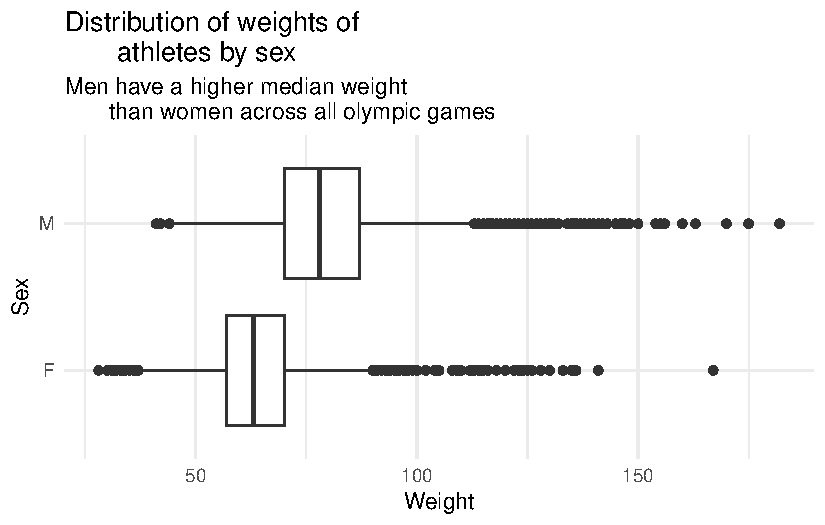
\includegraphics{project_files/figure-pdf/unnamed-chunk-6-1.pdf}

}

\end{figure}

As we can see from the boxplots above, the distribution of weight for
men and \women athletes competing in the olympics are both skewed to the
right, while it appears that the men are skewed heavier. We were
interested in the one female athlete who is considered an outlier
because her weight is above 150. We have found the athlete to be Olha
Vasylivna Korobka who actually got a silver medal in the 2008 summer
games in weight lifting. (Code shown below).

\begin{Shaded}
\begin{Highlighting}[]
\NormalTok{olympics }\SpecialCharTok{\%\textgreater{}\%}
  \FunctionTok{filter}\NormalTok{(sex }\SpecialCharTok{==} \StringTok{"F"}\NormalTok{) }\SpecialCharTok{\%\textgreater{}\%}
  \FunctionTok{filter}\NormalTok{(weight }\SpecialCharTok{\textgreater{}} \DecValTok{150}\NormalTok{)}
\end{Highlighting}
\end{Shaded}

\begin{verbatim}
# A tibble: 1 x 15
     id name      sex     age height weight team  noc   games  year season city 
  <dbl> <chr>     <chr> <dbl>  <dbl>  <dbl> <chr> <chr> <chr> <dbl> <chr>  <chr>
1 62843 Olha Vas~ F        22    181    167 Ukra~ UKR   2008~  2008 Summer Beij~
# ... with 3 more variables: sport <chr>, event <chr>, medal <chr>
\end{verbatim}

Height vs Sex BoxPlots

\begin{Shaded}
\begin{Highlighting}[]
\FunctionTok{ggplot}\NormalTok{(olympics , }\AttributeTok{mapping =} \FunctionTok{aes}\NormalTok{(}\AttributeTok{x =}\NormalTok{height , }\AttributeTok{y =}\NormalTok{ sex )) }\SpecialCharTok{+} 
  \FunctionTok{geom\_boxplot}\NormalTok{() }\SpecialCharTok{+} 
  \FunctionTok{theme\_minimal}\NormalTok{() }\SpecialCharTok{+} 
  \FunctionTok{labs}\NormalTok{(}\AttributeTok{x =} \StringTok{"Height"}\NormalTok{, }\AttributeTok{y =} \StringTok{"Sex"}\NormalTok{, }\AttributeTok{title =} \StringTok{"Distribution of heights of athletes }
\StringTok{       by sex"}\NormalTok{, }\AttributeTok{subtitle =} \StringTok{"Men have a higher median height than women across}
\StringTok{       all olympic games"}\NormalTok{)}
\end{Highlighting}
\end{Shaded}

\begin{figure}[H]

{\centering 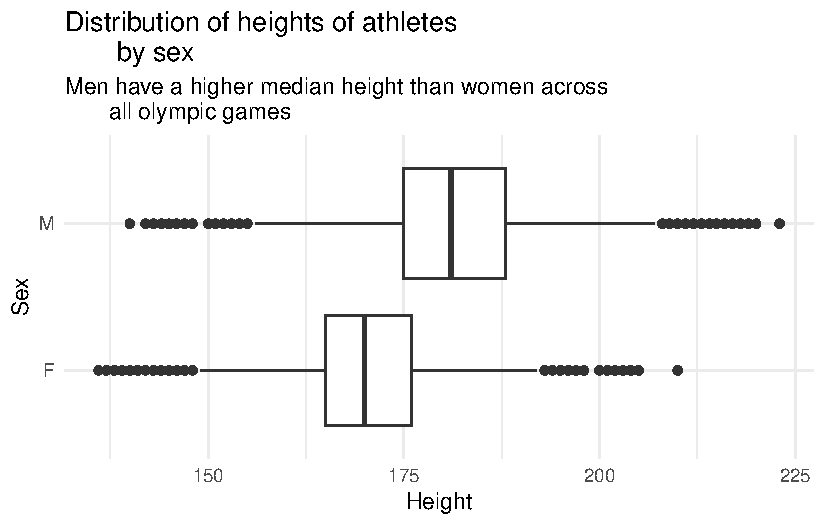
\includegraphics{project_files/figure-pdf/unnamed-chunk-8-1.pdf}

}

\end{figure}

Similar to the results that we saw in the boxplots comparing
distributions of weights between men and women, we can see that men also
have a higher median height than women who have completed in the
Olympics.

\emph{We chose to use all years when analyzing the distribution of
heights and weights} because over the course of our time frame (2004 -
2016) there have been many rule changes about allowed and not allowed
substances, and analyzing these two variables through all of the years
can give us a better idea of distributions.

Now that we have analyzed the data and got some idea of the distribution
of specific parameters of interest, we are interested in analyzing which
variables are the biggest factor in predicting gold medals for Summer
Olympic games, and whether or not these variables (and their influence)
change over time.

\hypertarget{logistic-regression}{%
\subsection{Logistic Regression}\label{logistic-regression}}

First we will fit a logistic regression model that predicts the
probability of receiving a gold medal (for the purpose of this model, we
will use the goldMedal? column that gives us a 1 if someone received a
gold medal for their event, and gives us a 0 if someone did not receive
a gold medal (they received either gold or silver) this is due to the
characteristics of logistic regression and how it works best when
predicting a binary outcome.)

\begin{verbatim}
# A tibble: 147 x 5
   term          estimate std.error  statistic p.value
   <chr>            <dbl>     <dbl>      <dbl>   <dbl>
 1 (Intercept) -15.0      624.      -0.0241     0.981 
 2 sexM          0.0535     0.0319   1.67       0.0942
 3 age           0.00165    0.00257  0.640      0.522 
 4 height        0.00201    0.00201  0.999      0.318 
 5 weight        0.000230   0.00148  0.156      0.876 
 6 nocALG       13.9      624.       0.0223     0.982 
 7 nocANZ        0.00897  764.       0.0000117  1.00  
 8 nocARG       13.9      624.       0.0222     0.982 
 9 nocARM       12.7      624.       0.0204     0.984 
10 nocAUS       13.6      624.       0.0217     0.983 
# ... with 137 more rows
\end{verbatim}

The expected log odds of someone achieving a gold medal if their sex is
male is 0.0535 times higher than if someone is a female when holding all
other variables constant. For every one year increase in age, the
expected log odds of someone achieving a gold medal is expected to
increase by .00164 when all other variables are held constant. For every
one unit increase in height, we expect the logs odds of someone
achieving a gold medal to increase by approximately 0.0020 when all
other variables are held constant. . For every one unit increase in
weight, we expect the log odds of someone achieving a gold medal to
increase by approximately 0.00022 when all other variables are held
constant. For each respective noc, the expected log odds of someone
achieving a gold medal to {[}increase or decrease{]} by X when all other
variables are held constant.

\hypertarget{ordinal-regression}{%
\subsection{Ordinal Regression}\label{ordinal-regression}}

\begin{verbatim}

Re-fitting to get Hessian
\end{verbatim}

\begin{verbatim}
# A tibble: 148 x 5
   term    estimate std.error statistic coef.type  
   <chr>      <dbl>     <dbl>     <dbl> <chr>      
 1 sexM   0.0227     0.0167      1.36   coefficient
 2 age    0.00128    0.00134     0.957  coefficient
 3 height 0.00126    0.00105     1.20   coefficient
 4 weight 0.0000409  0.000771    0.0531 coefficient
 5 nocALG 5.89       0.0254    232.     coefficient
 6 nocANZ 4.77       0.00141  3373.     coefficient
 7 nocARG 5.94       0.0768     77.3    coefficient
 8 nocARM 5.41       0.0217    249.     coefficient
 9 nocAUS 5.80       0.0364    160.     coefficient
10 nocAUT 5.85       0.0691     84.7    coefficient
# ... with 138 more rows
\end{verbatim}

\begin{Shaded}
\begin{Highlighting}[]
\FunctionTok{exp}\NormalTok{(}\FunctionTok{coef}\NormalTok{(ordMod))}
\end{Highlighting}
\end{Shaded}

\hypertarget{section}{%
\subsection{}\label{section}}

\hypertarget{variable-selection}{%
\subsection{Variable Selection}\label{variable-selection}}

\begin{Shaded}
\begin{Highlighting}[]
\NormalTok{y }\OtherTok{\textless{}{-}}\NormalTok{ olympics\_ord}\SpecialCharTok{$}\NormalTok{medals}
\NormalTok{x }\OtherTok{\textless{}{-}} \FunctionTok{model.matrix}\NormalTok{(medals }\SpecialCharTok{\textasciitilde{}}\NormalTok{ sex  }\SpecialCharTok{+}\NormalTok{ age }\SpecialCharTok{+}\NormalTok{ height }\SpecialCharTok{+}\NormalTok{  weight }\SpecialCharTok{+}\NormalTok{ noc ,}
                  \AttributeTok{data =}\NormalTok{ olympics\_ord)}
\NormalTok{m\_lasso\_cv }\OtherTok{\textless{}{-}} \FunctionTok{cv.glmnet}\NormalTok{(x, y, }\AttributeTok{alpha =} \DecValTok{1}\NormalTok{)}
\end{Highlighting}
\end{Shaded}

\begin{Shaded}
\begin{Highlighting}[]
\NormalTok{best\_lambda }\OtherTok{\textless{}{-}}\NormalTok{ m\_lasso\_cv}\SpecialCharTok{$}\NormalTok{lambda.min}
\NormalTok{best\_lambda}
\end{Highlighting}
\end{Shaded}

\begin{verbatim}
[1] 0.002823154
\end{verbatim}

\begin{Shaded}
\begin{Highlighting}[]
\FunctionTok{plot}\NormalTok{(m\_lasso\_cv)}
\end{Highlighting}
\end{Shaded}

\begin{figure}[H]

{\centering 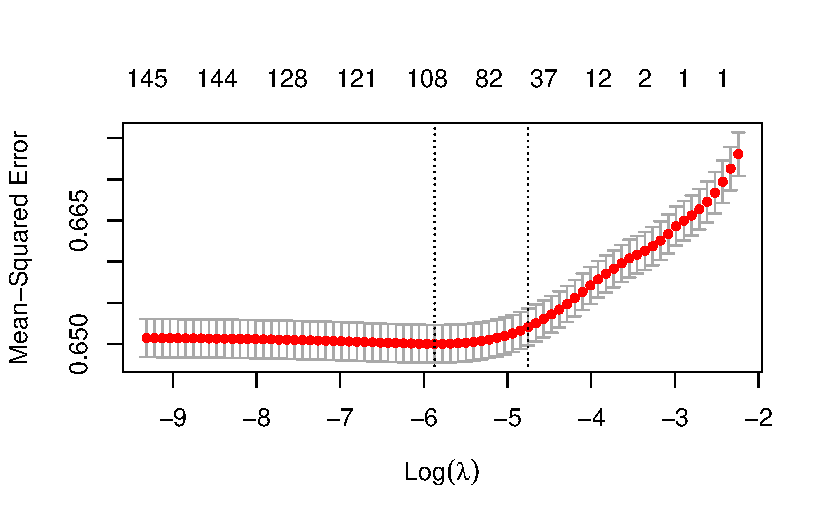
\includegraphics{project_files/figure-pdf/unnamed-chunk-15-1.pdf}

}

\end{figure}

\begin{Shaded}
\begin{Highlighting}[]
\NormalTok{m\_best }\OtherTok{\textless{}{-}} \FunctionTok{glmnet}\NormalTok{(x, y, }\AttributeTok{alpha =} \DecValTok{1}\NormalTok{, }\AttributeTok{lambda =}\NormalTok{ best\_lambda)}
\NormalTok{m\_best}\SpecialCharTok{$}\NormalTok{beta}
\end{Highlighting}
\end{Shaded}

\begin{Shaded}
\begin{Highlighting}[]
\FunctionTok{library}\NormalTok{(leaps)}
\NormalTok{m\_all\_noc }\OtherTok{\textless{}{-}} \FunctionTok{regsubsets}\NormalTok{(medals }\SpecialCharTok{\textasciitilde{}}\NormalTok{ sex  }\SpecialCharTok{+}\NormalTok{ age }\SpecialCharTok{+}\NormalTok{ height }\SpecialCharTok{+}\NormalTok{  weight }\SpecialCharTok{+}\NormalTok{ noc,}
                  \AttributeTok{data =}\NormalTok{ olympics\_ord, }
                  \AttributeTok{nbest =} \DecValTok{1}\NormalTok{, }\AttributeTok{nvmax =} \DecValTok{5}\NormalTok{, }\AttributeTok{really.big =}\NormalTok{ T)}
\NormalTok{m\_all\_noc}
\end{Highlighting}
\end{Shaded}

\begin{Shaded}
\begin{Highlighting}[]
\FunctionTok{summary}\NormalTok{(m\_all\_noc)}
\end{Highlighting}
\end{Shaded}

\begin{Shaded}
\begin{Highlighting}[]
\NormalTok{m\_all }\OtherTok{\textless{}{-}} \FunctionTok{regsubsets}\NormalTok{(medals }\SpecialCharTok{\textasciitilde{}}\NormalTok{ sex  }\SpecialCharTok{+}\NormalTok{ age }\SpecialCharTok{+}\NormalTok{ height }\SpecialCharTok{+}\NormalTok{  weight,}
                  \AttributeTok{data =}\NormalTok{ olympics\_ord, }
                  \AttributeTok{nbest =} \DecValTok{1}\NormalTok{, }\AttributeTok{nvmax =} \DecValTok{5}\NormalTok{, }\AttributeTok{really.big =}\NormalTok{ T)}
\NormalTok{m\_all}
\end{Highlighting}
\end{Shaded}

\begin{verbatim}
Subset selection object
Call: regsubsets.formula(medals ~ sex + age + height + weight, data = olympics_ord, 
    nbest = 1, nvmax = 5, really.big = T)
4 Variables  (and intercept)
       Forced in Forced out
sexM       FALSE      FALSE
age        FALSE      FALSE
height     FALSE      FALSE
weight     FALSE      FALSE
1 subsets of each size up to 4
Selection Algorithm: exhaustive
\end{verbatim}

\begin{Shaded}
\begin{Highlighting}[]
\FunctionTok{summary}\NormalTok{(m\_all)}
\end{Highlighting}
\end{Shaded}

\begin{verbatim}
Subset selection object
Call: regsubsets.formula(medals ~ sex + age + height + weight, data = olympics_ord, 
    nbest = 1, nvmax = 5, really.big = T)
4 Variables  (and intercept)
       Forced in Forced out
sexM       FALSE      FALSE
age        FALSE      FALSE
height     FALSE      FALSE
weight     FALSE      FALSE
1 subsets of each size up to 4
Selection Algorithm: exhaustive
         sexM age height weight
1  ( 1 ) " "  " " "*"    " "   
2  ( 1 ) " "  "*" "*"    " "   
3  ( 1 ) "*"  "*" "*"    " "   
4  ( 1 ) "*"  "*" "*"    "*"   
\end{verbatim}

\begin{Shaded}
\begin{Highlighting}[]
\FunctionTok{summary}\NormalTok{(m\_all)}\SpecialCharTok{$}\NormalTok{cp}
\end{Highlighting}
\end{Shaded}

\begin{verbatim}
[1] 8.033983 2.634207 3.027055 5.000000
\end{verbatim}

Final Model

\begin{Shaded}
\begin{Highlighting}[]
\NormalTok{ordMod\_final }\OtherTok{\textless{}{-}}
  \FunctionTok{polr}\NormalTok{(}\FunctionTok{factor}\NormalTok{(medals) }\SpecialCharTok{\textasciitilde{}}\NormalTok{ sex  }\SpecialCharTok{+}\NormalTok{ age }\SpecialCharTok{+}\NormalTok{ height , }\AttributeTok{data =}\NormalTok{ olympics\_ord , }\AttributeTok{method =} \StringTok{"probit"}\NormalTok{)}
\FunctionTok{tidy}\NormalTok{(ordMod\_final) }\SpecialCharTok{\%\textgreater{}\%}
  \FunctionTok{mutate}\NormalTok{(}\AttributeTok{estimate =} \FunctionTok{round}\NormalTok{(estimate , }\DecValTok{9}\NormalTok{))}
\end{Highlighting}
\end{Shaded}

\begin{verbatim}

Re-fitting to get Hessian
\end{verbatim}

\begin{verbatim}
# A tibble: 5 x 5
  term   estimate std.error statistic coef.type  
  <chr>     <dbl>     <dbl>     <dbl> <chr>      
1 sexM   -0.0196   0.0155      -1.27  coefficient
2 age    -0.00336  0.00129     -2.60  coefficient
3 height  0.00304  0.000673     4.52  coefficient
4 1|2     0.0192   0.118        0.163 scale      
5 2|3     0.863    0.118        7.30  scale      
\end{verbatim}

\hypertarget{results}{%
\subsection{Results}\label{results}}

LASSO removed weight as a variable and majority of all NOC identifiers
(country ) as variables as well. When we ran our all subset selection on
these variables, we got back the same data, which removed weight and
noc, leaving sex, age and height.

\hypertarget{discussion}{%
\subsection{Discussion}\label{discussion}}

In summary, we learned that weight does not have an impact on whether an
Olympian receives a gold medal or not. In addition, we learned that when
taking into consideration our variables of interest, sex age and height
are the only influential variables when we perform variable selection.\\
For our future work, we could subset this data by years and see if the
influence of these variables change over time. Additionally, we could
check the variable\textquotesingle s influence with
Cook\textquotesingle s Distance.

\hfill\break



\end{document}
